
\documentclass{article}

\usepackage[left=1.8cm,right=1.8cm, top=2cm, bottom = 2cm]{geometry}
\usepackage{amsfonts}

\usepackage{amsmath}
\usepackage{xcolor}

\usepackage{tikz}
\usepackage{subfigure}

\usepackage{pgfplots}

\pgfplotsset{compat=1.10}
\usepgfplotslibrary{fillbetween}
\usetikzlibrary{patterns}



\pagestyle{empty}

\setlength{\tabcolsep}{15pt}


\newcommand{\deriv}[3][]{\frac{\mathrm{d}^{#1}#2}{\mathrm{d}#3^{#1}}}
\newcommand{\diff}{\;\mathrm{d}}

\newcommand{\norm}[1]{\left|\kern-1pt\left|#1\right|\kern-1pt\right|}
\newcommand{\bra}[1]{\left\langle #1 \,\right|}
\newcommand{\ket}[1]{\left|\, #1\right\rangle}
\newcommand{\braket}[2]{\left\langle #1 \mid #2 \right\rangle}




\begin{document}

\title{Nyquist Plots}
\date{}

\maketitle
\thispagestyle{empty}

\Large

\vskip -10mm

\textbf{\underline{Objective: To sketch Nyquist plots and use them to test for closed-}}

\textbf{\underline{loop stability.}}



\vspace{5mm}



\textbf{Wamr-up: Contour Sketching:}\bigskip


Let $F$ be the complex-valued function
\[F(s)=\frac{1}{s+1}.\]

\begin{enumerate}
	\item Show that
		\[F(j\omega) = \frac{1-j\omega}{1+\omega^2}.\]
	\item Plot $F(j\omega)$ for $\omega=-3,-2,-1,0,1,2,3$ on an Argand diagram.
	\item Find
		\[\lim_{\omega\to \infty} F(j\omega)\]
		and
		\[\lim_{\omega\to -\infty} F(j\omega).\]
	\item Joining the points you plotted and using the limits calculated, sketch the curve $F(j\omega)$ as $\omega$ ranges over all real numbers. Include an arrow to indicate the direction of $\omega$ increasing.
	\item Show that for any $\omega$, $|F(j\omega)-0.5|=0.5$. What can you conclude about the shape of $F(j\omega)$?
\end{enumerate}







\clearpage


\textbf{Theory: Nyquist Plots:}\bigskip



Recall that the \textbf{frequency response} of a system is the Fourier transform of its impulse response; equivalently, it is the restriction of the transfer function to the imaginary axis ($s=j\omega)$. It describes the behaviour of a system for pure sinusoid inputs.

The transfer function $F$ is a complex-valued function, so for any $\omega$, $F(j\omega)$ is a complex number; this can be described by specifying its modulus and argument, which is what a Bode plot does, or by its real and imaginary parts; these can be conveniently displayed in an Argand diagram (plot of the complex plane). So for each $\omega$ we can plot the point $F(j\omega)$; this transforms the imaginary axis into a curve in the complex plane. This curve is called the \textbf{Nyquist plot} of $F$ (or of the system for which $F$ is the transfer function).

The Nyquist plot represents the same information as the Bode plot, but in a different form. The advantage of a Bode plot is that it is easy to read off both the modulus and argument (amplitude gain and phase shift) at a given frequency, which is harder on a Nyquist plot. The advantage of a Nyquist plot is that it is a single plot, rather than two linked plots, making it easier to see the overall behaviour of the frequency response as a whole. So, roughly speaking, the Bode plot is good for precise readings of the frequency response at specific frequencies, and the Nyquist plot for a general overview of the frequency response over all frequencies---the Bode plot gives the detail, and the Nyquist plot the big picture.\bigskip



Recall that if an open-loop system with transfer function $T(s)$ is given negative feedback with gain $F(s)$, then the closed-loop transfer function is
\[\frac{T(s)}{1+T(s)F(s)}.\]
This will have a new pole (beyond any that the original, open-loop system had) whenever $1+T(s)F(s)=0$; \textit{i.e.}, whenever $T(s)F(s)$ has modulus 1 and argument $\pi$ (equivalently $-\pi$). The \textbf{gain margin} is found by looking at when the phase is $\pi$ and taking the difference between the unstable gain of $1$ and the actual gain; it is how much the gain can be increased by without causing instability. This can be read off the Nyquist diagram by looking at the distance from $-1$ to the point where the Nyquist plot crosses the negative real axis (has argument $\pi$).

The \textbf{phase margin} is found by looking at when the gain is 1 and taking the difference between the unstable phase of $\pi$ and the actual phase. It is how much the phase shift could be changed by before causing an instability. This can be read off the Nyquist plot by finding the angle away from the negative real axis at the point where the Nyquist plot crosses the unit circle (has modulus 1).

\clearpage



\begin{center}
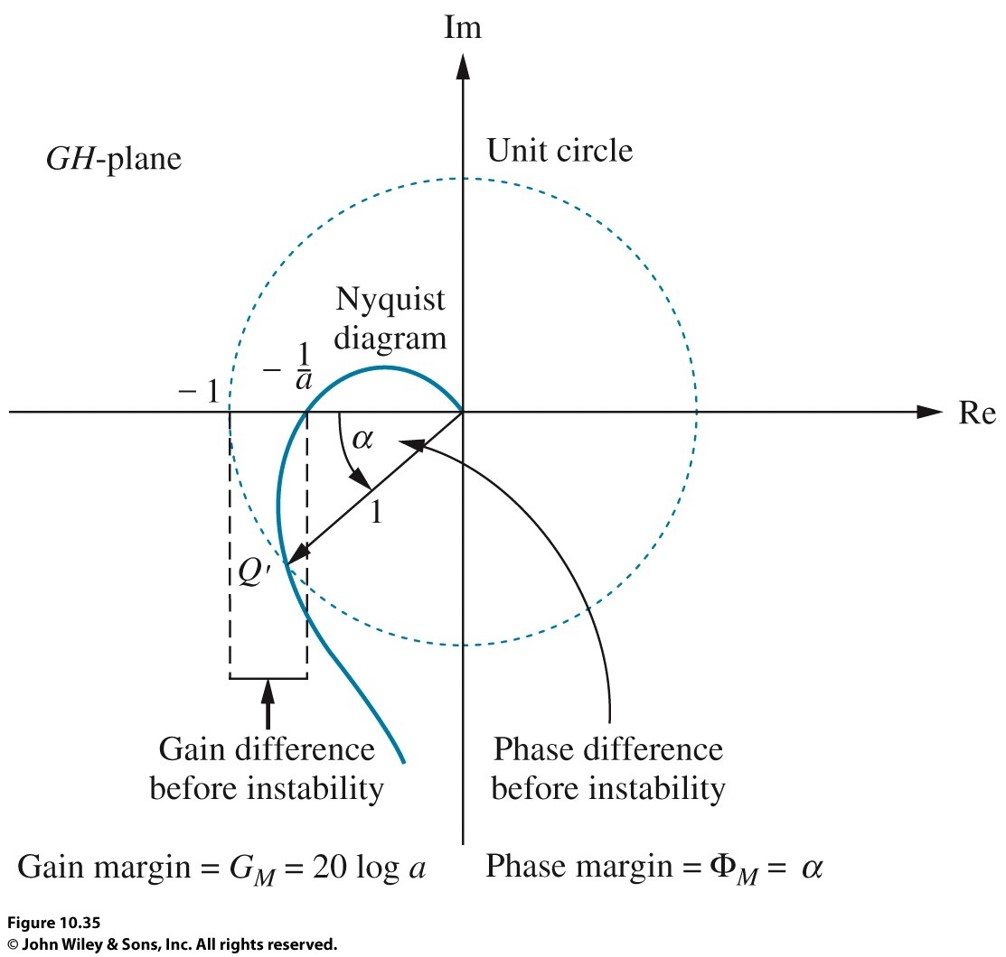
\includegraphics{NyquistGainPhase.jpg}
\end{center}



\clearpage



\textbf{Complex Analysis and Contour Integrals:}\bigskip



The Nyquist plot gives rise to a powerful tool for determining the stability of a closed-loop system from knowledge of the open-loop transfer function $T(s)$ and the feedback gain $F(s)$. This method, known as the \textbf{Nyquist stability criterion} is based on some rather difficult complex analysis. It requires knowledge of two deep results of calculus in the complex plane, called Cauchy's Argument Principle and Cauchy's Integral Formula. To cover the background theory for these results would take several weeks (at least!), so we will only look at a rough outline of the ideas.

Central to the argument is the notion of a \textbf{contour integral} in the complex plane. The idea is to take a curve in the complex plane, and a function defined over that curve, and to integrate the function over the curve. Recall that the integral of a function is the area under its graph, found by approximating the area by rectangles, and taking the limit as the number of rectangles tends to infinity and their width tends to 0.

So far we have only looked at functions over a straight axis, but we can consider integrating a function over a curve. Think of a shower curtain; we have a rail at the top, which is often straight, but for some showers is curved. As we draw the curtain, it curves to follow the rail, but the curtain itself still has a meaningful area. We can imagine dividing the rail into a sequence of short segments, each approximately straight, and drawing a rectangle below each segment which approximates the area of the shower curtain. We then take the limit, as for integrals on a straight axis, and find the area of the curtain. So an integral over a curved path is really no different to an integral over the $x$-axis; it's just that the area we are finding is of a curved shape, instead of a flat one.

When the curve $C$ we are integrating over is closed (\textit{i.e.}, has no loose ends---it meets back up with itself) we call the integral a contour integral, and denote it with the special symbol
\[\oint_C.\]
But it is really not very different to the integrals we've seen plenty of before.\bigskip


\textbf{Examples:}\medskip

Let $C$ be the unit circle, oriented anticlockwise. Compute
\[\oint_C e^s\diff s \qquad \mbox{and }\qquad\frac{1}{2\pi j}\oint_C \frac{1}{s}\diff s.\]

\clearpage




\textbf{Cauchy's Integral Theorems:}\bigskip



The Cauchy Argument Principle and Integral Formula are a pair of remarkable results about contour integrals. The argument principle says that given a simple (not self-intersecting) closed contour $C$ (oriented anticlockwise) and a complex, differentiable function $F(s)$, then
\[\frac{1}{2\pi j}\oint_C \frac{F'(s)}{F(s)}\diff s = Z-P,\]
where $Z$ is the number of zeroes of $F$ enclosed by $C$, and $P$ the number of poles enclosed by $C$. For instance, if $F(s)=s$, then $\frac{F'(s)}{F(s)}=\frac{1}{s}$; since $F(s)$ has one zero and no poles inside the unit circle, we expect that the integral of $\frac{1}{s}$, once divided by $2\pi j$, should be equal to 1. Indeed, this is exactly what we saw on the examples above!\bigskip

\textbf{Example:}\medskip

Let $C$ be the ellipse with foci at $1$ and $-2j$, oriented anticlockwise. By multiplying top and bottom by $e^{7s^2}$, evaluate
\[\oint_C \frac{14s^2-14s+1}{s-1}\diff s.\]

\vfill


The Cauchy Integral Formula has a few different forms; the version we shall need is that if $C$ is an anticlockwise-oriented, closed curve, but not necessarily simple (it may self-intersect), then
\[\frac{1}{2\pi j}\oint_C \frac{1}{s-a}\diff s\]
is the \textbf{winding number} of $C$ about the point $a$---the number of times $C$ wraps completely around $a$ anticlockwise, minus the number of times it wraps around clockwise.





\clearpage



\textbf{The Nyquist Stability Criterion:}\bigskip


Using Cauchy's Argument Principle and Integral Formula, we can study the number of poles of a closed-loop transfer function with positive real part. If $T(s)$ is the open-loop transfer function and $F(s)$ the (negative) feedback gain, then
\[\frac{T(s)}{1+T(s)F(s)}\]
is the closed-loop transfer function. Any new poles of this are zeros of $1+T(s)F(s)$. For convenience, write $D(s)=1+T(s)F(s)$.

Let $C$ be a contour which consists of going along the imaginary axis from $-Nj$ to $Nj$, then round in a large semicircle (clockwise) back to $-Nj$. The semicircle must be taken large enough to enclose all poles and zeros of $T(s)F(s)$ in the right-hand half-plane. By the Argument Principle,
\[-\frac{1}{2\pi j}\oint_C \frac{D'(s)}{D(s)}=Z-P,\]
where $Z$ is the number of zeros and $P$ the number of poles of $D(s)$ in the right-hand half-plane. Applying a change of variables $u=T(s)F(s)=D(s)-1$ to the integral, we have
\begin{align*}
	-\frac{1}{\pi j}\oint_{\Gamma} \frac{D'(s)}{u+1}\deriv{s}{u}\diff u&=-\frac{1}{2\pi j}\oint_\Gamma \frac{D'(s)}{u+1}\frac{1}{D'(s)}\diff u\\
	&=-\frac{1}{2\pi j}\oint_\Gamma \frac{1}{u+1}\diff u,
\end{align*}
where $\Gamma$ is the curve obtained from applying $T(s)F(s)$ to $C$, and where we have used
\[\deriv{u}{s}=D'(s)\quad \Rightarrow\quad \deriv{s}{u}=\frac{1}{D'(s)}.\]

Now Cauchy's Integral Formula tells us that this integral is exactly the winding number of $\Gamma$ about the point $-1$; call this $w_\Gamma(-1)$. So we have
\[w_\Gamma(-1)=Z-P.\]

Now, $P$ is the number of poles of $D(s)=1+T(s)F(s)$ in the right-hand half-plane, which is simply the number of poles of $T(s)F(s)$ in the RHHP. Meanwhile, $Z$ is the number of zeros of $D(s)$, hence the number of new poles of the closed-loop transfer function---the number we want to know! So, rearranging,
\[Z=P+w_\Gamma(-1).\]

\clearpage


\textbf{The Nyquist Stability Criterion (cont.):}\bigskip


That is, the number of new poles in the RHHP (new instabilities) is equal to the number of open-loop poles in the RHHP, plus the winding number of $\Gamma$ about $-1$. This depends on the curve $\Gamma$, which is obtained from the semicircle $C$ by applying $T(s)F(s)$; but the radius $N$ of $C$ can be taken as large as we like, and in the limit as $N\to\infty$, $C$ becomes just the imaginary axis, and so $\Gamma$ is exactly the Nyquist plot of $T(s)F(s)$.\bigskip

So to determine the number of new unstable poles of a closed-loop system, take the number of unstable poles of the open-loop system and subtract the number of anticlockwise windings of the Nyquist plot around $-1$.\bigskip


\textbf{Example:}\medskip


A system has open-loop transfer function
\[T(s)=\frac{10(s+1)(s+2)}{(s-3)(s-4)}.\]

When given unity-gain negative feedback, the Nquist plot is:
\begin{center}
	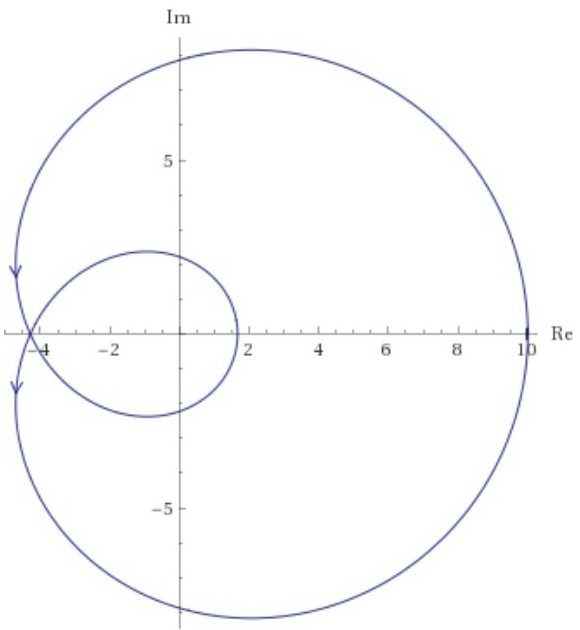
\includegraphics[scale=0.5]{NyquistExampleCropped.jpg}
\end{center}

Show that the closed-loop system is stable.

Note that the open-loop system in this case is not stable! This gives an example of how adding feedback can stabilise an unstable system, and how Nyquist's criterion can be used to see this.











\end{document}